%% Report on decays and LFV rates in the soft-broken S3-3HDM vacuum.
%% Companion: derivations_06.tex (the derivation ledger, auto-generated by the notebook).
%% Source: research/thdm_s3/06_soft_decays.ipynb
\documentclass[11pt,a4paper]{article}
\usepackage[T1]{fontenc}
\usepackage[utf8]{inputenc}
\usepackage{amsmath,amssymb}
\usepackage{graphicx}
\usepackage{booktabs}
\usepackage[margin=2.4cm]{geometry}
\usepackage[colorlinks=true,linkcolor=blue,citecolor=blue,urlcolor=blue]{hyperref}
\setlength{\parindent}{0pt}
\setlength{\parskip}{0.6em}

\title{Decays and LFV Higgs rates in the soft-broken $S_3$ 3HDM:\\
an exact lepton fit at any vacuum, and LFV as pure\\
non-vacuum admixture}
\author{M. Zeleny-Mora\\[2pt]
\small Instituto de Física, Universidad Nacional Autónoma de México}
\date{\today}

\begin{document}
\maketitle

\begin{abstract}
\noindent
I have computed the LFV Higgs rates, $h\to\gamma\gamma$ and the heavy-state decays
$A\to Zh$, $H^\pm\to W^\pm h$ at all 2021 viable points of the soft-broken scan. In this
vacuum the CP-even mixing is a full $3\times3$, so the single angle $\delta$ of the
exact-$S_3$ analysis no longer applies. Every coupling is computed numerically per point and
validated against \texttt{feynlag}'s own extractor at a non-aligned point, against the
exact-$S_3$ limit, and against the $S_3$ image vacuum. Three results stand out. First, the
charged-lepton fit is exact at any vacuum: the mass matrix is orthogonally an arrowhead, so
the fit is one cubic per sign pattern. Away from $\varphi=\pi/3$ the draft-type solution
survives only for $|\mu_3^\ell|\approx m_\tau$. Second, the vacuum direction's lepton coupling
is $\mathrm{diag}(m_\ell)/v$ at every vacuum, so the SM-like state's flavour violation is
carried entirely by its $1-\kappa_V^2$ admixture. Third, all three LFV channels open up, with
$h\to e\mu$ the binding one, yet only 5 of 2021 scalar points are excluded for every lepton
configuration.
\end{abstract}

\section{Summary}

Everything below comes from \texttt{research/thdm\_s3/06\_soft\_decays.ipynb}, with the
numerics in \texttt{soft\_decays.py} and \texttt{lfv.py}.

\begin{enumerate}\itemsep2pt
\item \textbf{Validated couplings} (\S\ref{sec:valid}): numeric $hH^+H^-$ and VSS couplings
agree with the extractor, the exact limit and the $S_3$ image.
\item \textbf{The lepton fit off the alignment} is an exact cubic, and soft breaking pins
$\mu_3^\ell$ near $\pm m_\tau$ (\S\ref{sec:lepton}).
\item \textbf{SM-like LFV is pure admixture}, and $e\mu$ is the binding channel
(\S\ref{sec:lfv}).
\item \textbf{$h\to\gamma\gamma$ and VSS} (\S\ref{sec:gg}).
\end{enumerate}

Doing this surfaced an error in the exact-vacuum analysis: its lepton Yukawa split had
$G_2=0$, which put the gauge-phobic $h_0$'s couplings in the wrong place. That is corrected in
the companion scalar-decays report. With the fix, $h_0$ couples only through the electron,
exactly as our draft prints.

\section{Validation}
\label{sec:valid}

The soft terms are quadratic, so a cubic coupling comes from the quartics alone. The
$h_kH^+_aH^-_b$ couplings are the lambdified tensor $\partial^3V/\partial r\,\partial c\,
\partial\bar c$ contracted with each point's rotations. Every doublet has the same gauge
charges, so the VSS couplings are pure geometry:
\[
g_{ZA_ah_k}=\frac{g}{2c_W}\,(R_{\rm odd}^{\mathsf T}R_{\rm even})_{ak},\qquad
g_{WH^\pm_ah_k}=\frac g2\,(R_C^{\mathsf T}R_{\rm even})_{ak}.
\]

\begin{center}
\begin{tabular}{lll}
\toprule
check & against & agreement\\
\midrule
27 $h_kH^+_aH^-_b$ couplings, soft point & \texttt{feynlag} extractor & $2\times10^{-13}$ GeV\\
9 $ZAh$ + 9 $WH^\pm h$ couplings & \texttt{feynlag} extractor & $10^{-17}$\\
$\Gamma(A\to Zh)$ closed form & decay engine $|M|^2$ & $10^{-10}$ relative\\
$\varphi=\pi/3$, zero soft terms & corrected notebook 03 & gauge-phobic state, trilinears, LFV\\
$\varphi\to2\pi/3-\varphi$ (40 points) & itself & $10^{-12}$\\
\bottomrule
\end{tabular}
\end{center}

\section{The charged-lepton fit off the alignment}
\label{sec:lepton}

In feynlag's basis the doublet block of $M_\ell$ is $a\mathbb 1+b\,v_{12}\,\mathrm{refl}(\varphi)$,
whose eigenvectors $e_\pm$ depend on $\varphi$ only. The third column projects on them as
$D(\cos\tfrac{3\varphi}2,\sin\tfrac{3\varphi}2)$, so
\[
M_\ell\simeq\begin{pmatrix}A&0&D\cos\chi\\0&B&D\sin\chi\\D\cos\chi&D\sin\chi&\mu_3\end{pmatrix},
\qquad\chi=\tfrac{3\varphi}2 .
\]
Matching the characteristic polynomial to $\prod_i(\lambda-s_im_i)$ leaves one cubic in
$A-B$ per sign pattern. Every branch is verified against the lepton masses. Random-start least
squares never finds a solution the cubic misses (377 converged fits). At $\varphi=\pi/3$,
$\cos\chi=0$ and the electron decouples, which recovers the draft. Existence depends on
$\cos3\varphi$ only.

\begin{figure}[h]
\centering
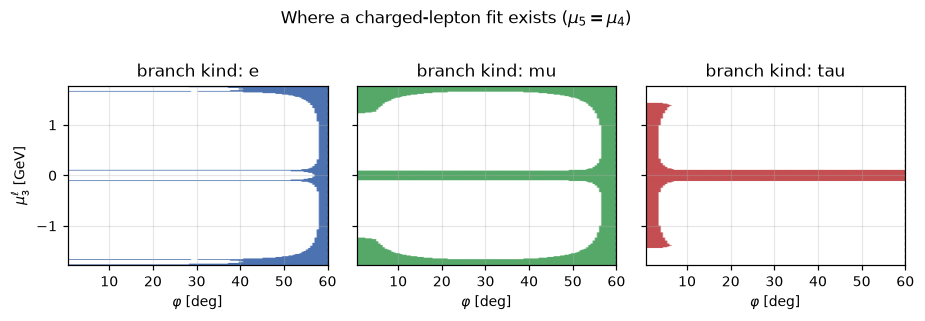
\includegraphics[width=0.95\textwidth]{figures/softdec_mu3_existence.png}
\caption{Where a lepton fit exists, by branch kind (which lepton the $e_+$ entry $A$ grows
into; ``e'' is the draft's branch). At $\varphi=60^\circ$ the whole $\mu_3$ axis is allowed.
Away from it the draft-type branch survives on about 5\% of the axis, near $\pm m_\tau$.}
\end{figure}

So soft breaking turns the exact model's free dial $\mu_3^\ell\in(m_\mu,m_\tau)$ into a
near-prediction: the third generation is essentially the $S_3$ singlet.

\section{LFV rates}
\label{sec:lfv}

The vacuum direction $\hat v$ couples to leptons through $\sum_kv_kG_k/v=M_\ell/v$, which is
diagonal in the mass basis at \emph{any} vacuum (checked to $10^{-17}$ at 203 points). The
SM-like state's flavour violation therefore comes entirely from its admixture of the other
two directions, of weight $1-\kappa_V^2$ (median $2.4\times10^{-3}$). This is the alignment
limit, and it holds whatever the size of the soft breaking (Fig.~\ref{fig:lfv}).

\begin{figure}[h]
\centering
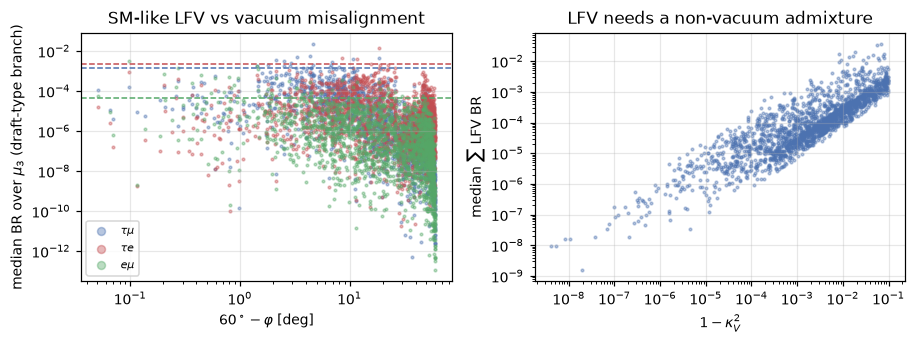
\includegraphics[width=0.95\textwidth]{figures/softdec_lfv.png}
\caption{Left: SM-like LFV rates (median over $\mu_3$, draft-type branch) against the vacuum
misalignment, with the CMS limits dashed. Right: the total LFV rate against the non-vacuum
admixture $1-\kappa_V^2$; the correlation is 0.88 in log.}
\label{fig:lfv}
\end{figure}

Over every (point, $\mu_3$, branch) entry, with $\Gamma_h=4.1$~MeV:

\begin{center}
\begin{tabular}{lccc}
\toprule
SM-like channel & median $\mathcal B$ & entries over the limit & limit (95\% CL)\\
\midrule
$\tau\mu$ & $9.4\times10^{-6}$ & 2.9\% & $1.5\times10^{-3}$ \cite{CMS21}\\
$\tau e$ & $9.3\times10^{-6}$ & 1.9\% & $2.2\times10^{-3}$ \cite{CMS21}\\
$e\mu$ & $2.6\times10^{-6}$ & \textbf{18.3\%} & $4.4\times10^{-5}$ \cite{CMS23}\\
\bottomrule
\end{tabular}
\end{center}

$e\mu$ binds hardest. Still, only \textbf{5 of 2021} scalar points have no lepton
configuration under all three limits. As at the exact vacuum, LFV data bound the lepton
parameters rather than the scalar sector.

\section{$h\to\gamma\gamma$ and the heavy states}
\label{sec:gg}

$R_{\gamma\gamma}=\Gamma/\Gamma_{\rm SM}$ uses both charged Higgses in the loop, with
coefficient $g_{hH^+H^-}v/(2m_{H^\pm}^2)$ \cite{ChakrabortiEtAl21}, and the top coupling
\emph{assumed} equal to $\kappa_V$. The median is 0.97, and 90\% of points lie in
$[0.85,1.00]$. The 48 points below 0.8 all have a light $H^\pm$ (below 310~GeV) interfering
destructively with the $W$. The charged loop decouples to $\kappa_V^2$ above 1.5~TeV.

\begin{figure}[h]
\centering
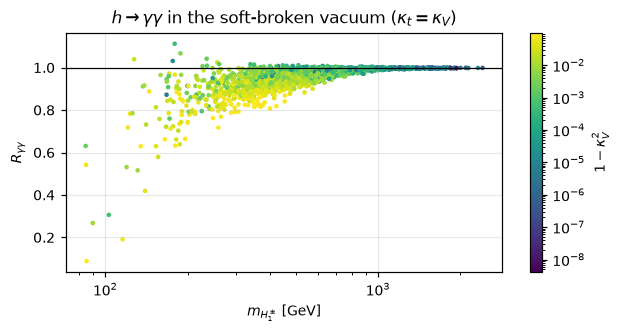
\includegraphics[width=0.70\textwidth]{figures/softdec_gammagamma.png}
\caption{$R_{\gamma\gamma}$ against the lighter charged-Higgs mass, coloured by the
non-vacuum admixture.}
\end{figure}

$A_{1,2}\to Zh$ and $H^\pm_{1,2}\to W^\pm h$ are open at nearly every point, with median
widths of 20--80~MeV. Their couplings to the SM-like state obey
$\sum_a|O_{ak}|^2=1-\kappa_V^2$ exactly, so they vanish in the alignment limit as $hVV$
saturates.

\section{Open questions}

\begin{enumerate}\itemsep4pt
\item \textbf{The quark sector per point.} The heavy-state total widths and the top coupling
in $R_{\gamma\gamma}$ both need it. The soft quark fit exists at one vacuum only.
\item \textbf{$R_{\gamma\gamma}$ as a cut.} It needs the production side and a cited signal
strength.
\item \textbf{$\mu\to e\gamma$.} Off the exact vacuum the $e\mu$ and $e\tau$ couplings are on,
and the radiative decays will likely constrain more than $h\to e\mu$.
\item \textbf{The $\mu_3$ prior.} The quoted fractions are over a uniform $\mu_3$ grid and all
branches; the 5-point exclusion count is prior-independent.
\end{enumerate}

\begin{thebibliography}{9}

\bibitem{LFVHD} M.~Zeleny-Mora, M.~Mondragón and T.~A.~Valencia-Pérez,
\emph{Exploring LFV Higgs decays in the Three Higgs Doublet Model}, draft
(\texttt{paper\_lfvhd/LFVHD\_3HDMS3.tex}).

\bibitem{CMS21} CMS Collaboration,
\emph{Search for lepton-flavor violating decays of the Higgs boson in the $\mu\tau$ and
$e\tau$ final states in pp collisions at $\sqrt s=13$~TeV},
Phys.\ Rev.\ D \textbf{104}, 032013 (2021),
\href{https://arxiv.org/abs/2105.03007}{arXiv:2105.03007}.

\bibitem{CMS23} CMS Collaboration,
\emph{Search for the lepton-flavor violating decay of the Higgs boson and additional Higgs
bosons in the $e\mu$ final state in proton-proton collisions at $\sqrt s=13$~TeV},
Phys.\ Rev.\ D \textbf{108}, 072004 (2023),
\href{https://arxiv.org/abs/2305.18106}{arXiv:2305.18106},
\href{https://doi.org/10.1103/PhysRevD.108.072004}{doi:10.1103/PhysRevD.108.072004}.

\bibitem{ChakrabortiEtAl21} M.~Chakraborti, D.~Das, M.~Levy, S.~Mukherjee and I.~Saha,
\emph{Prospects of light charged scalars in a three Higgs doublet model with $Z_3$
symmetry}, \href{https://arxiv.org/abs/2104.08146}{arXiv:2104.08146}.

\end{thebibliography}

\end{document}
